Soit $f$ une fonction définie et dérivable sur l'intervalle $[0\,;\,4]$, dont la courbe représentative $\mathcal{C}_f$ est représentée ci-dessous.

La droite $T$ est la tangente à la courbe au point d'abscisse 3.

\begin{minipage}{0.60\textwidth}
\begin{enumerate}
\item Par lecture graphique, déterminer :
\begin{enumerate}
\item L'image de 3 par la fonction $f$.
\item Le nombre dérivé $f'(3)$.
\end{enumerate}
\item Soit la fonction $f$ définie sur l'intervalle $[0\,;\,4]$ par :
\[
f(x)=-x^3+9x^2-24x+16
\]
\begin{enumerate}
\item Calculer $f(0)$.
\item Soit $f'$ la fonction dérivée de la fonction $f$.

Calculer $f'(x)$ pour tout réel $x$ de l'intervalle $[0\,;\,4]$, en détaillant les calculs.

\item Vérifier que pour tout réel $x$,
\[f'(x)=-3(x-2)(x-4).\]
\end{enumerate}
\end{enumerate}
\end{minipage}
\hfill
\begin{minipage}{0.40\textwidth}
\begin{center}
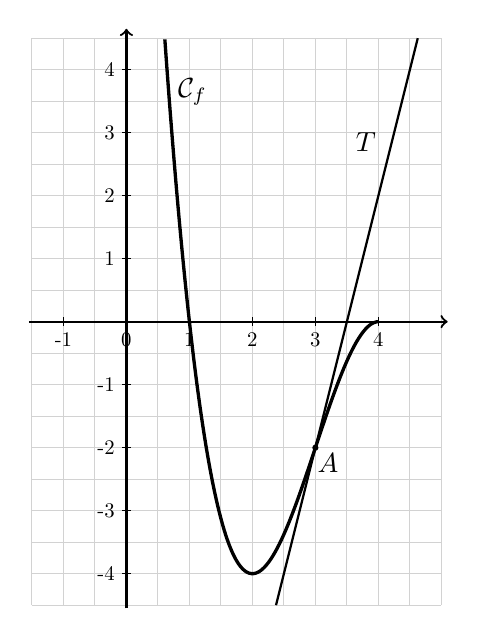
\begin{tikzpicture}[scale=0.8]
\draw[step=0.5,gray!35,thin] (-1.5,-4.5) grid (5,4.5);
\draw[->,thick] (-1.55,0)--(5.1,0);
\draw[->,thick] (0,-4.55)--(0,4.65);
\foreach \x in {-1,0,1,2,3,4} {\draw (\x,0.07)--(\x,-0.07) node[below,scale=0.75] {\x};}
\foreach \y in {-4,-3,-2,-1,1,2,3,4} {\draw (0.07,\y)--(-0.07,\y) node[left,scale=0.75] {\y};}
\draw[black,very thick,domain=0.61:4,samples=100,smooth] plot (\x,{-\x^3+9*\x^2-24*\x+16});
\draw[black,thick,domain=2.375:4.625] plot (\x,{4*\x-14});
\node at (1.05,3.65) {$\mathcal{C}_f$};
\node at (3.80,2.85) {$T$};
\node at (3.2,-2.25) {$A$};
\fill (3,-2) circle (1.4pt);
\end{tikzpicture}
\end{center}
\end{minipage}

\begin{enumerate}
\item[]
\begin{enumerate}[start=4]
\item Étudier le signe de $f'(x)$ et établir le tableau de variation de la fonction $f$ sur l'intervalle $[0\,;\,4]$, en y faisant figurer les extrémums.

\item Quel est le minimum de la fonction $f$ sur l'intervalle $[0\,;\,4]$ ?

En quelle valeur est-il atteint ?
\end{enumerate}
\end{enumerate}
